% Options for packages loaded elsewhere
\PassOptionsToPackage{unicode}{hyperref}
\PassOptionsToPackage{hyphens}{url}
%
\documentclass[
]{article}
\usepackage{amsmath,amssymb}
\usepackage{lmodern}
\usepackage{ifxetex,ifluatex}
\ifnum 0\ifxetex 1\fi\ifluatex 1\fi=0 % if pdftex
  \usepackage[T1]{fontenc}
  \usepackage[utf8]{inputenc}
  \usepackage{textcomp} % provide euro and other symbols
\else % if luatex or xetex
  \usepackage{unicode-math}
  \defaultfontfeatures{Scale=MatchLowercase}
  \defaultfontfeatures[\rmfamily]{Ligatures=TeX,Scale=1}
\fi
% Use upquote if available, for straight quotes in verbatim environments
\IfFileExists{upquote.sty}{\usepackage{upquote}}{}
\IfFileExists{microtype.sty}{% use microtype if available
  \usepackage[]{microtype}
  \UseMicrotypeSet[protrusion]{basicmath} % disable protrusion for tt fonts
}{}
\makeatletter
\@ifundefined{KOMAClassName}{% if non-KOMA class
  \IfFileExists{parskip.sty}{%
    \usepackage{parskip}
  }{% else
    \setlength{\parindent}{0pt}
    \setlength{\parskip}{6pt plus 2pt minus 1pt}}
}{% if KOMA class
  \KOMAoptions{parskip=half}}
\makeatother
\usepackage{xcolor}
\IfFileExists{xurl.sty}{\usepackage{xurl}}{} % add URL line breaks if available
\IfFileExists{bookmark.sty}{\usepackage{bookmark}}{\usepackage{hyperref}}
\hypersetup{
  pdftitle={mind2},
  pdfauthor={Ariel Levy},
  hidelinks,
  pdfcreator={LaTeX via pandoc}}
\urlstyle{same} % disable monospaced font for URLs
\usepackage[margin=1in]{geometry}
\usepackage{color}
\usepackage{fancyvrb}
\newcommand{\VerbBar}{|}
\newcommand{\VERB}{\Verb[commandchars=\\\{\}]}
\DefineVerbatimEnvironment{Highlighting}{Verbatim}{commandchars=\\\{\}}
% Add ',fontsize=\small' for more characters per line
\usepackage{framed}
\definecolor{shadecolor}{RGB}{248,248,248}
\newenvironment{Shaded}{\begin{snugshade}}{\end{snugshade}}
\newcommand{\AlertTok}[1]{\textcolor[rgb]{0.94,0.16,0.16}{#1}}
\newcommand{\AnnotationTok}[1]{\textcolor[rgb]{0.56,0.35,0.01}{\textbf{\textit{#1}}}}
\newcommand{\AttributeTok}[1]{\textcolor[rgb]{0.77,0.63,0.00}{#1}}
\newcommand{\BaseNTok}[1]{\textcolor[rgb]{0.00,0.00,0.81}{#1}}
\newcommand{\BuiltInTok}[1]{#1}
\newcommand{\CharTok}[1]{\textcolor[rgb]{0.31,0.60,0.02}{#1}}
\newcommand{\CommentTok}[1]{\textcolor[rgb]{0.56,0.35,0.01}{\textit{#1}}}
\newcommand{\CommentVarTok}[1]{\textcolor[rgb]{0.56,0.35,0.01}{\textbf{\textit{#1}}}}
\newcommand{\ConstantTok}[1]{\textcolor[rgb]{0.00,0.00,0.00}{#1}}
\newcommand{\ControlFlowTok}[1]{\textcolor[rgb]{0.13,0.29,0.53}{\textbf{#1}}}
\newcommand{\DataTypeTok}[1]{\textcolor[rgb]{0.13,0.29,0.53}{#1}}
\newcommand{\DecValTok}[1]{\textcolor[rgb]{0.00,0.00,0.81}{#1}}
\newcommand{\DocumentationTok}[1]{\textcolor[rgb]{0.56,0.35,0.01}{\textbf{\textit{#1}}}}
\newcommand{\ErrorTok}[1]{\textcolor[rgb]{0.64,0.00,0.00}{\textbf{#1}}}
\newcommand{\ExtensionTok}[1]{#1}
\newcommand{\FloatTok}[1]{\textcolor[rgb]{0.00,0.00,0.81}{#1}}
\newcommand{\FunctionTok}[1]{\textcolor[rgb]{0.00,0.00,0.00}{#1}}
\newcommand{\ImportTok}[1]{#1}
\newcommand{\InformationTok}[1]{\textcolor[rgb]{0.56,0.35,0.01}{\textbf{\textit{#1}}}}
\newcommand{\KeywordTok}[1]{\textcolor[rgb]{0.13,0.29,0.53}{\textbf{#1}}}
\newcommand{\NormalTok}[1]{#1}
\newcommand{\OperatorTok}[1]{\textcolor[rgb]{0.81,0.36,0.00}{\textbf{#1}}}
\newcommand{\OtherTok}[1]{\textcolor[rgb]{0.56,0.35,0.01}{#1}}
\newcommand{\PreprocessorTok}[1]{\textcolor[rgb]{0.56,0.35,0.01}{\textit{#1}}}
\newcommand{\RegionMarkerTok}[1]{#1}
\newcommand{\SpecialCharTok}[1]{\textcolor[rgb]{0.00,0.00,0.00}{#1}}
\newcommand{\SpecialStringTok}[1]{\textcolor[rgb]{0.31,0.60,0.02}{#1}}
\newcommand{\StringTok}[1]{\textcolor[rgb]{0.31,0.60,0.02}{#1}}
\newcommand{\VariableTok}[1]{\textcolor[rgb]{0.00,0.00,0.00}{#1}}
\newcommand{\VerbatimStringTok}[1]{\textcolor[rgb]{0.31,0.60,0.02}{#1}}
\newcommand{\WarningTok}[1]{\textcolor[rgb]{0.56,0.35,0.01}{\textbf{\textit{#1}}}}
\usepackage{graphicx}
\makeatletter
\def\maxwidth{\ifdim\Gin@nat@width>\linewidth\linewidth\else\Gin@nat@width\fi}
\def\maxheight{\ifdim\Gin@nat@height>\textheight\textheight\else\Gin@nat@height\fi}
\makeatother
% Scale images if necessary, so that they will not overflow the page
% margins by default, and it is still possible to overwrite the defaults
% using explicit options in \includegraphics[width, height, ...]{}
\setkeys{Gin}{width=\maxwidth,height=\maxheight,keepaspectratio}
% Set default figure placement to htbp
\makeatletter
\def\fps@figure{htbp}
\makeatother
\setlength{\emergencystretch}{3em} % prevent overfull lines
\providecommand{\tightlist}{%
  \setlength{\itemsep}{0pt}\setlength{\parskip}{0pt}}
\setcounter{secnumdepth}{-\maxdimen} % remove section numbering
\ifluatex
  \usepackage{selnolig}  % disable illegal ligatures
\fi

\title{mind2}
\author{Ariel Levy}
\date{6/12/2018}

\begin{document}
\maketitle

Este trabalho original de \emph{Michael C. Frank} (Stanford University)
encontra-se em

\href{https://www.youtube.com/watch?v=qvPDE4ppAns\&t=757s}{mind 2017
vídeo}

e

\href{https://github.com/Data-on-the-Mind/2017-summer-workshop}{mind
2017 Github}

e do capítulo 5 (3 na versão impressa) do livro texto
\href{http://r4ds.had.co.nz/}{R4DS} Wickham e Grolemund (2016).

\hypertarget{objetivos-e-introduuxe7uxe3o}{%
\section{Objetivos e Introdução}\label{objetivos-e-introduuxe7uxe3o}}

Ao fim deste tutorial vocês entenderão o que é ``tidy data''

\begin{itemize}
\item
  Porque usar o tideverse leva a um formato bem inreressante de
  trabalho.
\item
  Como obter o que se deseja neste formato `tidy'
\item
  Como colocar seus dados neste formato
\item
  E algumas dicas e truques para lidar com dados em R.
\end{itemize}

Vamos explorar o pacote tidyverse e ter uma visão geral do R e do
RStudio utilizando inicialmente um conjunto de dados famoso, dataframe,
denominado IRIS que vem com o pacote ggplot2.

\hypertarget{data-frame-ou-tibble}{%
\subsection{Data frame ou tibble}\label{data-frame-ou-tibble}}

Data frames tem linhas e colunas e cada coluna tem um tipo distinto.
Iris é um banco de dados que mostra um conjunto de medidas de diferentes
instâncias de flores do tipo iris de diferentes espécies.

\begin{Shaded}
\begin{Highlighting}[]
\FunctionTok{head}\NormalTok{(iris)}
\end{Highlighting}
\end{Shaded}

\begin{verbatim}
##   Sepal.Length Sepal.Width Petal.Length Petal.Width Species
## 1          5.1         3.5          1.4         0.2  setosa
## 2          4.9         3.0          1.4         0.2  setosa
## 3          4.7         3.2          1.3         0.2  setosa
## 4          4.6         3.1          1.5         0.2  setosa
## 5          5.0         3.6          1.4         0.2  setosa
## 6          5.4         3.9          1.7         0.4  setosa
\end{verbatim}

\begin{Shaded}
\begin{Highlighting}[]
\FunctionTok{as.tibble}\NormalTok{(iris)}
\end{Highlighting}
\end{Shaded}

\begin{verbatim}
## # A tibble: 150 x 5
##    Sepal.Length Sepal.Width Petal.Length Petal.Width Species
##           <dbl>       <dbl>        <dbl>       <dbl> <fct>  
##  1          5.1         3.5          1.4         0.2 setosa 
##  2          4.9         3            1.4         0.2 setosa 
##  3          4.7         3.2          1.3         0.2 setosa 
##  4          4.6         3.1          1.5         0.2 setosa 
##  5          5           3.6          1.4         0.2 setosa 
##  6          5.4         3.9          1.7         0.4 setosa 
##  7          4.6         3.4          1.4         0.3 setosa 
##  8          5           3.4          1.5         0.2 setosa 
##  9          4.4         2.9          1.4         0.2 setosa 
## 10          4.9         3.1          1.5         0.1 setosa 
## # ... with 140 more rows
\end{verbatim}

R é uma linguagem mutio flexível uma vantagem, mas poode ser também uma
fraqueza já que as muitas formas de obter uma variável pode ser confuso
quando se misturam as formas.

Por exemplo vamos fazer um exercício de obter o terceiro valor a
terceira linha do data set.

\begin{Shaded}
\begin{Highlighting}[]
\NormalTok{iris}\SpecialCharTok{$}\NormalTok{Petal.Length[}\DecValTok{3}\NormalTok{]}
\end{Highlighting}
\end{Shaded}

\begin{verbatim}
## [1] 1.3
\end{verbatim}

\begin{Shaded}
\begin{Highlighting}[]
\NormalTok{iris[}\DecValTok{3}\NormalTok{,}\DecValTok{3}\NormalTok{]}
\end{Highlighting}
\end{Shaded}

\begin{verbatim}
## [1] 1.3
\end{verbatim}

\begin{Shaded}
\begin{Highlighting}[]
\NormalTok{iris[[}\StringTok{"Petal.Length"}\NormalTok{]][}\DecValTok{3}\NormalTok{]}
\end{Highlighting}
\end{Shaded}

\begin{verbatim}
## [1] 1.3
\end{verbatim}

\begin{Shaded}
\begin{Highlighting}[]
\NormalTok{iris[}\DecValTok{3}\NormalTok{,}\StringTok{"Petal.Length"}\NormalTok{]}
\end{Highlighting}
\end{Shaded}

\begin{verbatim}
## [1] 1.3
\end{verbatim}

Você pode acessar uma coluna usando \$ como em: `iris\$Petal.Length'

ou tratar o data frame como uma matriz e fazer `iris{[}3,3{]}',

ou ainda como uma lista e `iris{[}{[}``Petal.Length''{]}{]}{[}3{]}'

ou combinando as formas como em `iris{[}3,``Petal.Length''{]}'

\textbf{Porque algumas formas são melhores que outras?}

\begin{itemize}
\item
  Saber o tipo de variável em cada coluna
\item
  Trabalhar de forma programática
\item
  Leitura do código por humanos
\end{itemize}

\textbf{``Tidy datasets are all alike, but ver messy dataset is messy in
its own way'' - Hadley Wickham}

Se cada coluna representa uma \textbf{variável} e cada linha uma
\textbf{observação} com um \textbf{valor} então este é um conjunto de
dados organizado (tidy).

Se os dados estão assim organizados pode-se fazer coisas
programaticamente de forma uniforme. (R4DS).

Quando os dados estão armazenados de forma organizada a facilidade do R
de trabalhar vetorizadamente avolumasse. Fica fácil de entender os
verbos que traduzem operações uniformes.

Iris é um conjunto de dados organizado (tidy).

Cada coluna contém uma variável e cada linha uma observação. Uma
estrutura consistente.

\hypertarget{funuxe7uxf5es-pipes}{%
\subsection{Funções \& Pipes}\label{funuxe7uxf5es-pipes}}

Tudo que você quer tipicamente fazer em programação estatística utiliza
uma função (y=f(x)). A média (mean) é um bom exemplo utiliza um
argumento (x) que será do tipo vetor numérico.

\begin{Shaded}
\begin{Highlighting}[]
\FunctionTok{mean}\NormalTok{(iris}\SpecialCharTok{$}\NormalTok{Petal.Length)}
\end{Highlighting}
\end{Shaded}

\begin{verbatim}
## [1] 3.758
\end{verbatim}

Nós vamos denominar isso \textbf{aplicar}, em inglês `apply', a função
média (mean) ao vetor `Petal.Length'.

Pipes (CMD+shift+M para IOS ou CTRL+shift+M) é um modo de criar
sentenças com funções de forma mais simples. Ao colocar primeiro o
argumento da função. Então você escreverá:

\begin{Shaded}
\begin{Highlighting}[]
\NormalTok{iris}\SpecialCharTok{$}\NormalTok{Petal.Length }\SpecialCharTok{\%\textgreater{}\%}\NormalTok{ mean}
\end{Highlighting}
\end{Shaded}

\begin{verbatim}
## [1] 3.758
\end{verbatim}

Isso será particularmente útil quando encardearmos as funções.

\begin{Shaded}
\begin{Highlighting}[]
\FunctionTok{mean}\NormalTok{(}\FunctionTok{unique}\NormalTok{(iris}\SpecialCharTok{$}\NormalTok{Petal.Length))}
\end{Highlighting}
\end{Shaded}

\begin{verbatim}
## [1] 4.22093
\end{verbatim}

\begin{Shaded}
\begin{Highlighting}[]
\NormalTok{iris}\SpecialCharTok{$}\NormalTok{Petal.Length }\SpecialCharTok{\%\textgreater{}\%}\NormalTok{ unique }\SpecialCharTok{\%\textgreater{}\%}\NormalTok{ mean}
\end{Highlighting}
\end{Shaded}

\begin{verbatim}
## [1] 4.22093
\end{verbatim}

ou

\begin{Shaded}
\begin{Highlighting}[]
\FunctionTok{round}\NormalTok{(}\FunctionTok{mean}\NormalTok{(}\FunctionTok{unique}\NormalTok{(iris}\SpecialCharTok{$}\NormalTok{Petal.Length)), }\AttributeTok{digits =} \DecValTok{2}\NormalTok{)}
\end{Highlighting}
\end{Shaded}

\begin{verbatim}
## [1] 4.22
\end{verbatim}

\begin{Shaded}
\begin{Highlighting}[]
\NormalTok{iris}\SpecialCharTok{$}\NormalTok{Petal.Length }\SpecialCharTok{\%\textgreater{}\%}\NormalTok{ unique }\SpecialCharTok{\%\textgreater{}\%}\NormalTok{ mean }\SpecialCharTok{\%\textgreater{}\%} \FunctionTok{round}\NormalTok{(}\AttributeTok{digits =} \DecValTok{2}\NormalTok{)}
\end{Highlighting}
\end{Shaded}

\begin{verbatim}
## [1] 4.22
\end{verbatim}

\begin{Shaded}
\begin{Highlighting}[]
\CommentTok{\# indenting makes things even easier to read}
\NormalTok{iris}\SpecialCharTok{$}\NormalTok{Petal.Length }\SpecialCharTok{\%\textgreater{}\%} 
\NormalTok{  unique }\SpecialCharTok{\%\textgreater{}\%} 
\NormalTok{  mean }\SpecialCharTok{\%\textgreater{}\%} 
  \FunctionTok{round}\NormalTok{(}\AttributeTok{digits =} \DecValTok{2}\NormalTok{)}
\end{Highlighting}
\end{Shaded}

\begin{verbatim}
## [1] 4.22
\end{verbatim}

Este modo de escrever torna a leitura e compreensão do código mais
fáceis.

Vamos utilizar muito este operador e voc6es verão como é simples.

\textbf{Exercício:}

Reescreva o comando abaixo usando o operador \%\textgreater\%

\begin{Shaded}
\begin{Highlighting}[]
\FunctionTok{length}\NormalTok{(}\FunctionTok{unique}\NormalTok{(iris}\SpecialCharTok{$}\NormalTok{Species)) }\CommentTok{\# number of species}
\end{Highlighting}
\end{Shaded}

\begin{verbatim}
## [1] 3
\end{verbatim}

\#\#ggplot2 \& tidyverse

Como verificamos em nossas aulas anteriores a visualização dos dados tem
papel importante na análise de dados.

De modo simplificado podemos rever duas partes importantes:

\begin{itemize}
\item
  aes - a estética e o mapeamento leva a segmentação das variáveis (x,
  y, cor, sí,bolo, etc.)
\item
  geom- o objeto geométrico que representará os dados( pontos, linhas,
  formas, etc.)
\end{itemize}

E apenas para apresentar algumas de minhas preferências eu gosto do
theme\_few do pacote ggthemes e a escala de cor solar\_color\_solarized.

\begin{Shaded}
\begin{Highlighting}[]
\FunctionTok{ggplot}\NormalTok{(iris, }\FunctionTok{aes}\NormalTok{(Sepal.Width, Sepal.Length, }\AttributeTok{col =}\NormalTok{ Species)) }\SpecialCharTok{+} 
  \FunctionTok{geom\_point}\NormalTok{() }\SpecialCharTok{+} 
\NormalTok{  ggthemes}\SpecialCharTok{::}\FunctionTok{theme\_few}\NormalTok{() }\SpecialCharTok{+} 
\NormalTok{  ggthemes}\SpecialCharTok{::}\FunctionTok{scale\_color\_solarized}\NormalTok{() }
\end{Highlighting}
\end{Shaded}

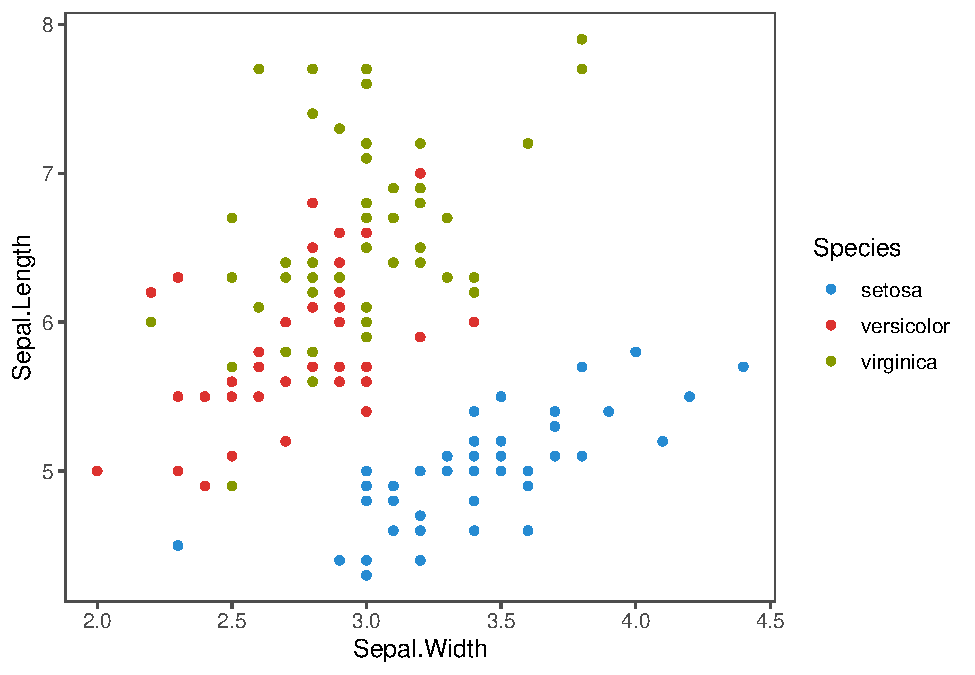
\includegraphics{mind2_files/figure-latex/unnamed-chunk-9-1.pdf}

\emph{\emph{Para casa:}}

Verifique outras paletas de cores e themas e eleja seu preferido.

** De volta a transformação dos dados **

\begin{Shaded}
\begin{Highlighting}[]
\FunctionTok{library}\NormalTok{(nycflights13)}
\end{Highlighting}
\end{Shaded}

Este novo conjunto de dados será utilizado para, como no livro texto
\emph{R4DS}, apresentar os principais ``verbos'' que correspondem aos
processos de transformações dos dados.

Estes dados, do pacote \emph{dplr} descrevem os voos que partiram da
cidade de Nova York em 2013. Estes dados tem como fonte o
\href{https://www.transtats.bts.gov/DatabaseInfo.asp?DB_ID=120\&Link=0}{US
Bureau of Tansportation Statistics}.

\begin{Shaded}
\begin{Highlighting}[]
\NormalTok{flights}
\end{Highlighting}
\end{Shaded}

\begin{verbatim}
## # A tibble: 336,776 x 19
##     year month   day dep_time sched_dep_time dep_delay arr_time sched_arr_time
##    <int> <int> <int>    <int>          <int>     <dbl>    <int>          <int>
##  1  2013     1     1      517            515         2      830            819
##  2  2013     1     1      533            529         4      850            830
##  3  2013     1     1      542            540         2      923            850
##  4  2013     1     1      544            545        -1     1004           1022
##  5  2013     1     1      554            600        -6      812            837
##  6  2013     1     1      554            558        -4      740            728
##  7  2013     1     1      555            600        -5      913            854
##  8  2013     1     1      557            600        -3      709            723
##  9  2013     1     1      557            600        -3      838            846
## 10  2013     1     1      558            600        -2      753            745
## # ... with 336,766 more rows, and 11 more variables: arr_delay <dbl>,
## #   carrier <chr>, flight <int>, tailnum <chr>, origin <chr>, dest <chr>,
## #   air_time <dbl>, distance <dbl>, hour <dbl>, minute <dbl>, time_hour <dttm>
\end{verbatim}

\textbf{Tipos de variáveis}

\begin{itemize}
\item
  int corresponde a inteiros.
\item
  dbl corresponde a double, ou números reais.
\item
  chr corresponde a vetores de caracteres.
\item
  dttm corresponde a data e hora (uma data + um horário).
\end{itemize}

Neste conjunto de dados temos só estes mas outros irão aparecer ao longo
do curso.

\hypertarget{o-buxe1sico-do-dplyr}{%
\subsubsection{O Básico do dplyr}\label{o-buxe1sico-do-dplyr}}

Este pacote presta-se a transformação dos dados, com estas
transformações resolve-se a maioria das questões envolvendo manipulação
dos dados:

\begin{itemize}
\item
  filter ( ) seleciona as observações por valores.
\item
  arrange ( ) reordena as linhas.
\item
  select ( ) seleciona as variáveis pelos nomes.
\item
  mutate ( ) cria novas variáveis com funções das variáveis existentes
\item
  sumarise ( ) reduz as estatísticas a poucos valores.
\end{itemize}

Normalmente utiliza-se junto a \emph{group-by ( )} que modifica o escopo
da função aos subconjuntos dos dados processando grupo por grupo. Estes
seis verbos estabelecem uma linguagem para a manipulação de dados.

Todos os verbos operam de forma similar:

\begin{enumerate}
\def\labelenumi{\arabic{enumi}.}
\item
  O primeiro argumento é um conjunto de dados.
\item
  Os argumentos subsequentes descrevem o que fazer com o conjunto de
  dados, utilizando o nome das vaiáveis sem aspas.
\item
  O resultado é um novo conjunto de dados.
\end{enumerate}

\hypertarget{filter}{%
\paragraph{Filter ( )}\label{filter}}

filter ( ) seleciona as observações por valores. Por exemplo, vamos
selecionar todos os voos de 01/janeiro/2013, com a instrução:

filter(flights, month == 1, day == 1)

mas como o \emph{dplyr} nunca altera o conjunto original ao executar um
processo você deverá atribuir o resultado a um novo objeto com
\textless- (Windows/Linux: ``Alt'' + ``-'', Mac: ``Option'' + ``-'', no
console ou chunk).

\begin{Shaded}
\begin{Highlighting}[]
\NormalTok{(jan1 }\OtherTok{\textless{}{-}} \FunctionTok{filter}\NormalTok{(flights, month }\SpecialCharTok{==} \DecValTok{12}\NormalTok{, day }\SpecialCharTok{==} \DecValTok{25}\NormalTok{))}
\end{Highlighting}
\end{Shaded}

\begin{verbatim}
## # A tibble: 719 x 19
##     year month   day dep_time sched_dep_time dep_delay arr_time sched_arr_time
##    <int> <int> <int>    <int>          <int>     <dbl>    <int>          <int>
##  1  2013    12    25      456            500        -4      649            651
##  2  2013    12    25      524            515         9      805            814
##  3  2013    12    25      542            540         2      832            850
##  4  2013    12    25      546            550        -4     1022           1027
##  5  2013    12    25      556            600        -4      730            745
##  6  2013    12    25      557            600        -3      743            752
##  7  2013    12    25      557            600        -3      818            831
##  8  2013    12    25      559            600        -1      855            856
##  9  2013    12    25      559            600        -1      849            855
## 10  2013    12    25      600            600         0      850            846
## # ... with 709 more rows, and 11 more variables: arr_delay <dbl>,
## #   carrier <chr>, flight <int>, tailnum <chr>, origin <chr>, dest <chr>,
## #   air_time <dbl>, distance <dbl>, hour <dbl>, minute <dbl>, time_hour <dttm>
\end{verbatim}

O parenteses externo tem a função de forçar o R a tanto o commando como
o resultado se estivéssemos utilizando um script ou no console.

\hypertarget{comparauxe7uxf5es}{%
\subsubsection{Comparações}\label{comparauxe7uxf5es}}

Para usar o \emph{filter ( )} você deve dominar os operadores de
comparação do R.

O R disponibiliza um conjunto padrão: \textgreater, \textgreater=,
\textless, \textless=, != (não igual) e = (igual).

Quando você inicia no R é comum fazer o erro de utilizar = ao invés de
== ao testar uma igualdade.

\begin{Shaded}
\begin{Highlighting}[]
\FunctionTok{filter}\NormalTok{(flights, }\AttributeTok{month=}\DecValTok{1}\NormalTok{)}
\end{Highlighting}
\end{Shaded}

Também podes ter problemas se utilizar == com números reais. Em
operações como:

\[(\sqrt(2))^2==2\]\\
ou

\[ \frac{1}{49}*49==1\]

\begin{Shaded}
\begin{Highlighting}[]
\FunctionTok{sqrt}\NormalTok{(}\DecValTok{2}\NormalTok{) }\SpecialCharTok{\^{}} \DecValTok{2} \SpecialCharTok{==} \DecValTok{2}
\end{Highlighting}
\end{Shaded}

\begin{verbatim}
## [1] FALSE
\end{verbatim}

\begin{Shaded}
\begin{Highlighting}[]
\DecValTok{1}\SpecialCharTok{/}\DecValTok{49} \SpecialCharTok{*} \DecValTok{49} \SpecialCharTok{==} \DecValTok{1}
\end{Highlighting}
\end{Shaded}

\begin{verbatim}
## [1] FALSE
\end{verbatim}

Nestes casos utilize \emph{near ( )}, computadores fazem contas com
aproximações e muitas casas decimais ( neste caso se atrapalham com os
algoritmos).

no R

\begin{Shaded}
\begin{Highlighting}[]
\FunctionTok{near}\NormalTok{(}\FunctionTok{sqrt}\NormalTok{(}\DecValTok{2}\NormalTok{)}\SpecialCharTok{\^{}}\DecValTok{2}\NormalTok{, }\DecValTok{2}\NormalTok{)}
\end{Highlighting}
\end{Shaded}

\begin{verbatim}
## [1] TRUE
\end{verbatim}

\begin{Shaded}
\begin{Highlighting}[]
\FunctionTok{near}\NormalTok{(}\DecValTok{1}\SpecialCharTok{/}\DecValTok{49} \SpecialCharTok{*} \DecValTok{49}\NormalTok{, }\DecValTok{1}\NormalTok{)}
\end{Highlighting}
\end{Shaded}

\begin{verbatim}
## [1] TRUE
\end{verbatim}

** Operadores Lógicos**

No R é comum a utilização dos operadores booleanos:

\& é e, \textbar{} é ou, ! é não,

\begin{figure}
\centering
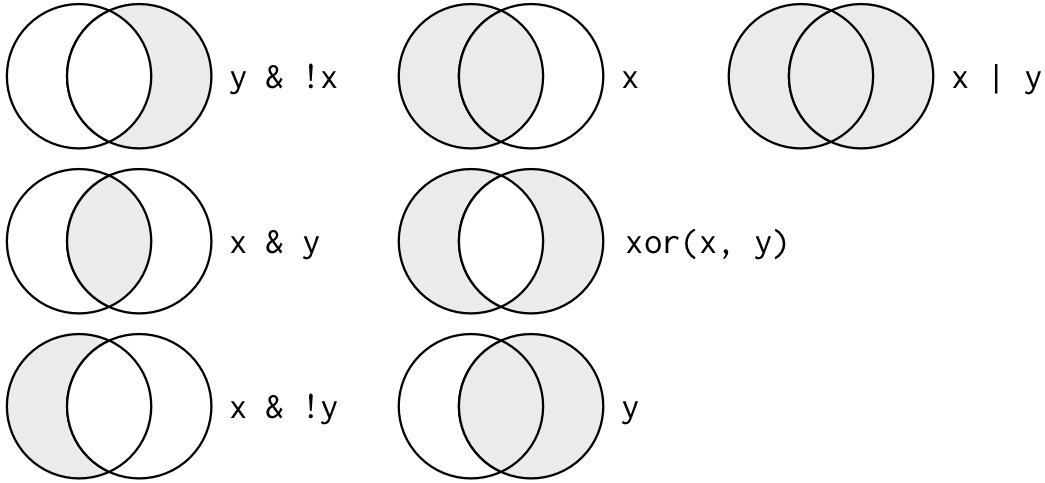
\includegraphics{/Users/alevy/Desktop/R4DS/Figs/transform-logical.png}
\caption{Operadores lógicos}
\end{figure}

Agora imagine o resultado desta expressão

filter(flights, month == 11 \textbar{} 12)

\begin{Shaded}
\begin{Highlighting}[]
\FunctionTok{filter}\NormalTok{(flights, month }\SpecialCharTok{==} \DecValTok{11} \SpecialCharTok{|}\NormalTok{ month }\SpecialCharTok{==} \DecValTok{12}\NormalTok{)}
\end{Highlighting}
\end{Shaded}

\begin{verbatim}
## # A tibble: 55,403 x 19
##     year month   day dep_time sched_dep_time dep_delay arr_time sched_arr_time
##    <int> <int> <int>    <int>          <int>     <dbl>    <int>          <int>
##  1  2013    11     1        5           2359         6      352            345
##  2  2013    11     1       35           2250       105      123           2356
##  3  2013    11     1      455            500        -5      641            651
##  4  2013    11     1      539            545        -6      856            827
##  5  2013    11     1      542            545        -3      831            855
##  6  2013    11     1      549            600       -11      912            923
##  7  2013    11     1      550            600       -10      705            659
##  8  2013    11     1      554            600        -6      659            701
##  9  2013    11     1      554            600        -6      826            827
## 10  2013    11     1      554            600        -6      749            751
## # ... with 55,393 more rows, and 11 more variables: arr_delay <dbl>,
## #   carrier <chr>, flight <int>, tailnum <chr>, origin <chr>, dest <chr>,
## #   air_time <dbl>, distance <dbl>, hour <dbl>, minute <dbl>, time_hour <dttm>
\end{verbatim}

Pode ser confuso, não?

Então uma outra forma seria utilizar \%in\% como em x \%in \%y
reescrevendo teremos:

\begin{Shaded}
\begin{Highlighting}[]
\NormalTok{nov\_dec}\OtherTok{\textless{}{-}}\FunctionTok{filter}\NormalTok{(flights, month }\SpecialCharTok{\%in\%} \FunctionTok{c}\NormalTok{(}\DecValTok{11}\NormalTok{,}\DecValTok{12}\NormalTok{))}
\end{Highlighting}
\end{Shaded}

\textbf{Lei de De Morgan }

!(x \& y) = !x \textbar{} !y

e

!(x \textbar{} y) = !x \& !y

O R tem também operadores condicionais \&\& e \textbar\textbar{} mas
aprenderemos mais sobre eles depois.

Quando você complicar os filtros com muitos operadores lógicos,
considere colocar as respostas em novas variáveis. Pode facilitar
bastante verificar os resultados depois.

\#\#Valores Faltantes\#\#

Quase sempre teremos valores faltantes nas bases de dados. No R são
representados por NA (não avaliado), NA representa um valor
desconhecido. Quase toda operação envolvendo NA retornará como resultado
NA. Assim, NA é contagioso!

Experimente:

\begin{Shaded}
\begin{Highlighting}[]
\ConstantTok{NA} \SpecialCharTok{\textgreater{}} \DecValTok{5}
\end{Highlighting}
\end{Shaded}

\begin{verbatim}
## [1] NA
\end{verbatim}

\begin{Shaded}
\begin{Highlighting}[]
\DecValTok{10} \SpecialCharTok{==} \ConstantTok{NA}
\end{Highlighting}
\end{Shaded}

\begin{verbatim}
## [1] NA
\end{verbatim}

\begin{Shaded}
\begin{Highlighting}[]
\ConstantTok{NA} \SpecialCharTok{+} \DecValTok{10}
\end{Highlighting}
\end{Shaded}

\begin{verbatim}
## [1] NA
\end{verbatim}

\begin{Shaded}
\begin{Highlighting}[]
\ConstantTok{NA} \SpecialCharTok{/} \DecValTok{2}
\end{Highlighting}
\end{Shaded}

\begin{verbatim}
## [1] NA
\end{verbatim}

\begin{Shaded}
\begin{Highlighting}[]
\NormalTok{(x}\OtherTok{\textless{}{-}}\ConstantTok{NA}\NormalTok{)}
\end{Highlighting}
\end{Shaded}

\begin{verbatim}
## [1] NA
\end{verbatim}

Para determinar se um valor é NA utilize is.na():

\begin{Shaded}
\begin{Highlighting}[]
\FunctionTok{is.na}\NormalTok{(x)}
\end{Highlighting}
\end{Shaded}

\begin{verbatim}
## [1] TRUE
\end{verbatim}

A instrução \emph{filter ( )} só responde para condições verdadeiras
(TRUE). Ela exclui NA e resultados falsos (FALSE).

\begin{Shaded}
\begin{Highlighting}[]
\NormalTok{(df}\OtherTok{\textless{}{-}}\FunctionTok{tibble}\NormalTok{(}\AttributeTok{x=}\NormalTok{(}\FunctionTok{c}\NormalTok{(}\FunctionTok{seq}\NormalTok{(}\DecValTok{1}\SpecialCharTok{:}\DecValTok{3}\NormalTok{),}\ConstantTok{NA}\NormalTok{))))}
\end{Highlighting}
\end{Shaded}

\begin{verbatim}
## # A tibble: 4 x 1
##       x
##   <int>
## 1     1
## 2     2
## 3     3
## 4    NA
\end{verbatim}

\begin{Shaded}
\begin{Highlighting}[]
\NormalTok{(}\FunctionTok{filter}\NormalTok{(df, x}\SpecialCharTok{\textgreater{}}\DecValTok{2}\NormalTok{))}
\end{Highlighting}
\end{Shaded}

\begin{verbatim}
## # A tibble: 1 x 1
##       x
##   <int>
## 1     3
\end{verbatim}

Se desejar manter os NA deverá especificat esta decisão por meio de um
teste lógico específico.

\begin{Shaded}
\begin{Highlighting}[]
\NormalTok{(}\FunctionTok{filter}\NormalTok{(df, x}\SpecialCharTok{\textgreater{}}\DecValTok{2} \SpecialCharTok{|} \FunctionTok{is.na}\NormalTok{(x)))}
\end{Highlighting}
\end{Shaded}

\begin{verbatim}
## # A tibble: 2 x 1
##       x
##   <int>
## 1     3
## 2    NA
\end{verbatim}

\textbf{Exercícios:} Escreva um Rmarkdown com o código de resposta dos
seguintes exercícios em que estejam presentes os enunciados e os
códigos. Poste no Schoology nos exercícios da aula de Dplyr realizados
em sala.

1- Encontre todos os voos que

\begin{enumerate}
\def\labelenumi{\alph{enumi}.}
\item
  Atrasaram a chegada duas horas ou mais.
\item
  Voaram para Houston (IAH ou HOU).
\item
  Foram operados pelas companhias United, American ou Delta.
\item
  Partiram entre meia noite e 6:00 a.m. (inclusive).
\end{enumerate}

2- O que faz a função auxiliar do dplyr \emph{between ( )}? Pode ser útl
para simplificar os códigos escritos? Mostre.

3- Quantos voos tem horário de partida faltando? Há outras variáveis
faltando? O que estas linhas provavelmente representam?

\#\#Ordenando as linhas com \emph{arrange ( )}\#\#

Muito similar ao \emph{filter ( )} exceto de que ao inv6es de selecionar
um subconjunto das linhas irá reordena-las.

Utiliza um conjunto de dados e uma lista de colunas ( ou expressões mais
complicadas) para ordenar.

Quando estiver utilizando mais de uma coluna, as demis serão utilizadas
nos desempates.

\begin{Shaded}
\begin{Highlighting}[]
\FunctionTok{arrange}\NormalTok{(flights, year, month, day)}
\end{Highlighting}
\end{Shaded}

\begin{verbatim}
## # A tibble: 336,776 x 19
##     year month   day dep_time sched_dep_time dep_delay arr_time sched_arr_time
##    <int> <int> <int>    <int>          <int>     <dbl>    <int>          <int>
##  1  2013     1     1      517            515         2      830            819
##  2  2013     1     1      533            529         4      850            830
##  3  2013     1     1      542            540         2      923            850
##  4  2013     1     1      544            545        -1     1004           1022
##  5  2013     1     1      554            600        -6      812            837
##  6  2013     1     1      554            558        -4      740            728
##  7  2013     1     1      555            600        -5      913            854
##  8  2013     1     1      557            600        -3      709            723
##  9  2013     1     1      557            600        -3      838            846
## 10  2013     1     1      558            600        -2      753            745
## # ... with 336,766 more rows, and 11 more variables: arr_delay <dbl>,
## #   carrier <chr>, flight <int>, tailnum <chr>, origin <chr>, dest <chr>,
## #   air_time <dbl>, distance <dbl>, hour <dbl>, minute <dbl>, time_hour <dttm>
\end{verbatim}

utilize \emph{desc ( )} para ordem descendente

\begin{Shaded}
\begin{Highlighting}[]
\FunctionTok{arrange}\NormalTok{(flights, }\FunctionTok{desc}\NormalTok{(arr\_delay))}
\end{Highlighting}
\end{Shaded}

\begin{verbatim}
## # A tibble: 336,776 x 19
##     year month   day dep_time sched_dep_time dep_delay arr_time sched_arr_time
##    <int> <int> <int>    <int>          <int>     <dbl>    <int>          <int>
##  1  2013     1     9      641            900      1301     1242           1530
##  2  2013     6    15     1432           1935      1137     1607           2120
##  3  2013     1    10     1121           1635      1126     1239           1810
##  4  2013     9    20     1139           1845      1014     1457           2210
##  5  2013     7    22      845           1600      1005     1044           1815
##  6  2013     4    10     1100           1900       960     1342           2211
##  7  2013     3    17     2321            810       911      135           1020
##  8  2013     7    22     2257            759       898      121           1026
##  9  2013    12     5      756           1700       896     1058           2020
## 10  2013     5     3     1133           2055       878     1250           2215
## # ... with 336,766 more rows, and 11 more variables: arr_delay <dbl>,
## #   carrier <chr>, flight <int>, tailnum <chr>, origin <chr>, dest <chr>,
## #   air_time <dbl>, distance <dbl>, hour <dbl>, minute <dbl>, time_hour <dttm>
\end{verbatim}

NA serão sempres dispostos ao final.

\textbf{Exercícios:}

4- Encontre os seis voos que mais chegaram mais atrasados.

5- Ordene o arquivo para encontrar os voos mais rápidos.

6 -Quais voos viajaram mais longe? E quais viajaram para mais perto?

\#\#Selecione as colunas com \emph{select ( )}\#\#

Não é incomum encontrar bases de dados com muitas variáveis. Nestes
casos um primeiro desafio é selecionar com quais variáveis se deseja
trabalhar.

\emph{select( )} permite criar um subconjunto apenas com as variáves
selecionadas.

escolha\textless-select(flights, year, month, day)

ou poderíamos escrever

escolha\textless-select(flights, year : day)

ou utilizar para excluir determinadas colunas

escolha\_menos\textless-select(flights,-(year : day))

Há diversas funções auxiliares para utilizar com \emph{select ( )}:

\begin{itemize}
\item
  \emph{starts\_with (``abc'')} encontra os nomes que começam com
  ``abc''.
\item
  \emph{ends\_with (``abc'')} encontra os nomes que terminam com
  ``abc''.
\item
  \emph{contains ( ``jlk'')} encontra os nomes que contém ``jlk''.
\item
  \emph{matches (``(.)//1'' )} encontra os nomes que atendem a
  determinadas condições. Esta encontra qualquer variável que contém
  caracteres repetidos. Vamos aprender mais depois.
\item
  \emph{num\_range (``x'', 1:3)} encontra x1,x2, e x3.
\end{itemize}

para renomear variáveis utilize \emph{rename( )}

\begin{Shaded}
\begin{Highlighting}[]
\FunctionTok{rename}\NormalTok{(flights, }\AttributeTok{tail\_num=}\NormalTok{tailnum)}
\end{Highlighting}
\end{Shaded}

\begin{verbatim}
## # A tibble: 336,776 x 19
##     year month   day dep_time sched_dep_time dep_delay arr_time sched_arr_time
##    <int> <int> <int>    <int>          <int>     <dbl>    <int>          <int>
##  1  2013     1     1      517            515         2      830            819
##  2  2013     1     1      533            529         4      850            830
##  3  2013     1     1      542            540         2      923            850
##  4  2013     1     1      544            545        -1     1004           1022
##  5  2013     1     1      554            600        -6      812            837
##  6  2013     1     1      554            558        -4      740            728
##  7  2013     1     1      555            600        -5      913            854
##  8  2013     1     1      557            600        -3      709            723
##  9  2013     1     1      557            600        -3      838            846
## 10  2013     1     1      558            600        -2      753            745
## # ... with 336,766 more rows, and 11 more variables: arr_delay <dbl>,
## #   carrier <chr>, flight <int>, tail_num <chr>, origin <chr>, dest <chr>,
## #   air_time <dbl>, distance <dbl>, hour <dbl>, minute <dbl>, time_hour <dttm>
\end{verbatim}

Selecione \emph{select()} junto com \emph{everythin()} para reordenar as
colunas como desejar, mantendo todas as demais.

\begin{Shaded}
\begin{Highlighting}[]
\FunctionTok{select}\NormalTok{(flights, time\_hour, air\_time, }\FunctionTok{everything}\NormalTok{())}
\end{Highlighting}
\end{Shaded}

\begin{verbatim}
## # A tibble: 336,776 x 19
##    time_hour           air_time  year month   day dep_time sched_dep_time
##    <dttm>                 <dbl> <int> <int> <int>    <int>          <int>
##  1 2013-01-01 05:00:00      227  2013     1     1      517            515
##  2 2013-01-01 05:00:00      227  2013     1     1      533            529
##  3 2013-01-01 05:00:00      160  2013     1     1      542            540
##  4 2013-01-01 05:00:00      183  2013     1     1      544            545
##  5 2013-01-01 06:00:00      116  2013     1     1      554            600
##  6 2013-01-01 05:00:00      150  2013     1     1      554            558
##  7 2013-01-01 06:00:00      158  2013     1     1      555            600
##  8 2013-01-01 06:00:00       53  2013     1     1      557            600
##  9 2013-01-01 06:00:00      140  2013     1     1      557            600
## 10 2013-01-01 06:00:00      138  2013     1     1      558            600
## # ... with 336,766 more rows, and 12 more variables: dep_delay <dbl>,
## #   arr_time <int>, sched_arr_time <int>, arr_delay <dbl>, carrier <chr>,
## #   flight <int>, tailnum <chr>, origin <chr>, dest <chr>, distance <dbl>,
## #   hour <dbl>, minute <dbl>
\end{verbatim}

\textbf{Exercícios:}

7- O que ocorre se você numa instrução \emph{select ( )} repetir uma
variável múltiplas vezes?

8- 0 que faz a função one\_of( )? Como poderia ser útil na utilização
com esse vetor? vars\textless-c(``year'',``month'',``day'',
``dep\_delay'',``arr\_delay'')

9- Como o reultado da execução do código abaixo o surpreendeu? Como
podes alterar o padrão da caixa alta e baixa? select(flights,
contains(``TIME''))

\#\#Adicionar novas variáveis com \emph{mutate ( )}\#\#

\begin{Shaded}
\begin{Highlighting}[]
\NormalTok{flights\_sml }\OtherTok{\textless{}{-}} \FunctionTok{select}\NormalTok{(flights, }
\NormalTok{  year}\SpecialCharTok{:}\NormalTok{day, }
  \FunctionTok{ends\_with}\NormalTok{(}\StringTok{"delay"}\NormalTok{), }
\NormalTok{  distance, }
\NormalTok{  air\_time}
\NormalTok{)}
\FunctionTok{mutate}\NormalTok{(flights\_sml,}
  \AttributeTok{gain =}\NormalTok{ arr\_delay }\SpecialCharTok{{-}}\NormalTok{ dep\_delay,}
  \AttributeTok{speed =}\NormalTok{ distance }\SpecialCharTok{/}\NormalTok{ air\_time }\SpecialCharTok{*} \DecValTok{60}
\NormalTok{)}
\end{Highlighting}
\end{Shaded}

\begin{verbatim}
## # A tibble: 336,776 x 9
##     year month   day dep_delay arr_delay distance air_time  gain speed
##    <int> <int> <int>     <dbl>     <dbl>    <dbl>    <dbl> <dbl> <dbl>
##  1  2013     1     1         2        11     1400      227     9  370.
##  2  2013     1     1         4        20     1416      227    16  374.
##  3  2013     1     1         2        33     1089      160    31  408.
##  4  2013     1     1        -1       -18     1576      183   -17  517.
##  5  2013     1     1        -6       -25      762      116   -19  394.
##  6  2013     1     1        -4        12      719      150    16  288.
##  7  2013     1     1        -5        19     1065      158    24  404.
##  8  2013     1     1        -3       -14      229       53   -11  259.
##  9  2013     1     1        -3        -8      944      140    -5  405.
## 10  2013     1     1        -2         8      733      138    10  319.
## # ... with 336,766 more rows
\end{verbatim}

Note que podes inclusive referir-se a colunas recém criadas.

\begin{Shaded}
\begin{Highlighting}[]
\FunctionTok{mutate}\NormalTok{(flights\_sml,}
  \AttributeTok{gain =}\NormalTok{ arr\_delay }\SpecialCharTok{{-}}\NormalTok{ dep\_delay,}
  \AttributeTok{hours =}\NormalTok{ air\_time }\SpecialCharTok{/} \DecValTok{60}\NormalTok{,}
  \AttributeTok{gain\_per\_hour =}\NormalTok{ gain }\SpecialCharTok{/}\NormalTok{ hours}
\NormalTok{)}
\end{Highlighting}
\end{Shaded}

\begin{verbatim}
## # A tibble: 336,776 x 10
##     year month   day dep_delay arr_delay distance air_time  gain hours
##    <int> <int> <int>     <dbl>     <dbl>    <dbl>    <dbl> <dbl> <dbl>
##  1  2013     1     1         2        11     1400      227     9 3.78 
##  2  2013     1     1         4        20     1416      227    16 3.78 
##  3  2013     1     1         2        33     1089      160    31 2.67 
##  4  2013     1     1        -1       -18     1576      183   -17 3.05 
##  5  2013     1     1        -6       -25      762      116   -19 1.93 
##  6  2013     1     1        -4        12      719      150    16 2.5  
##  7  2013     1     1        -5        19     1065      158    24 2.63 
##  8  2013     1     1        -3       -14      229       53   -11 0.883
##  9  2013     1     1        -3        -8      944      140    -5 2.33 
## 10  2013     1     1        -2         8      733      138    10 2.3  
## # ... with 336,766 more rows, and 1 more variable: gain_per_hour <dbl>
\end{verbatim}

Se desejar manter apenas as colunas criadas utiize \emph{transmute ( )}.

\begin{Shaded}
\begin{Highlighting}[]
\FunctionTok{transmute}\NormalTok{(flights,}
  \AttributeTok{gain =}\NormalTok{ arr\_delay }\SpecialCharTok{{-}}\NormalTok{ dep\_delay,}
  \AttributeTok{hours =}\NormalTok{ air\_time }\SpecialCharTok{/} \DecValTok{60}\NormalTok{,}
  \AttributeTok{gain\_per\_hour =}\NormalTok{ gain }\SpecialCharTok{/}\NormalTok{ hours}
\NormalTok{)}
\end{Highlighting}
\end{Shaded}

\begin{verbatim}
## # A tibble: 336,776 x 3
##     gain hours gain_per_hour
##    <dbl> <dbl>         <dbl>
##  1     9 3.78           2.38
##  2    16 3.78           4.23
##  3    31 2.67          11.6 
##  4   -17 3.05          -5.57
##  5   -19 1.93          -9.83
##  6    16 2.5            6.4 
##  7    24 2.63           9.11
##  8   -11 0.883        -12.5 
##  9    -5 2.33          -2.14
## 10    10 2.3            4.35
## # ... with 336,766 more rows
\end{verbatim}

\textbf{Funções úteis para criar com mutate}

\begin{itemize}
\item
  \emph{operadores aritméticos} +, -, *, /, \^{}. São de utilização
  vetorizada e também atendem a reciclagem.
\item
  \emph{módulo aritmético} \%/\% (inteiro da divisão) e \%\% (resto).
\end{itemize}

exemplo de utilização:

\begin{Shaded}
\begin{Highlighting}[]
\FunctionTok{transmute}\NormalTok{(flights,}
\NormalTok{  dep\_time,}
  \AttributeTok{hour =}\NormalTok{ dep\_time }\SpecialCharTok{\%/\%} \DecValTok{100}\NormalTok{,}
  \AttributeTok{minute =}\NormalTok{ dep\_time }\SpecialCharTok{\%\%} \DecValTok{100}
\NormalTok{)}
\end{Highlighting}
\end{Shaded}

\begin{verbatim}
## # A tibble: 336,776 x 3
##    dep_time  hour minute
##       <int> <dbl>  <dbl>
##  1      517     5     17
##  2      533     5     33
##  3      542     5     42
##  4      544     5     44
##  5      554     5     54
##  6      554     5     54
##  7      555     5     55
##  8      557     5     57
##  9      557     5     57
## 10      558     5     58
## # ... with 336,766 more rows
\end{verbatim}

\begin{itemize}
\item
  \emph{Logs}: log(), log2(), log10() são incrivelmente úteis mas vamos
  falar muito ainda neles. São especialmente importantes quando os dados
  tem amplitude sobre variada ordem de magnitude. Eles também convertem
  relações de produto em soma. Se utilizarem a base dois, log2 ( ) a
  interpretação fica facilitada já que a diferença de 1 na escala
  logarítma corresponderá ao dobro. E um a mesnos na diferença dos
  valore corresponde a metade.
\item
  \emph{Afastamentos}: lead() e lag() exemplos:
\end{itemize}

\begin{Shaded}
\begin{Highlighting}[]
\NormalTok{(x }\OtherTok{\textless{}{-}} \DecValTok{1}\SpecialCharTok{:}\DecValTok{10}\NormalTok{)}
\end{Highlighting}
\end{Shaded}

\begin{verbatim}
##  [1]  1  2  3  4  5  6  7  8  9 10
\end{verbatim}

\begin{Shaded}
\begin{Highlighting}[]
\FunctionTok{lag}\NormalTok{(x)}
\end{Highlighting}
\end{Shaded}

\begin{verbatim}
##  [1] NA  1  2  3  4  5  6  7  8  9
\end{verbatim}

\begin{Shaded}
\begin{Highlighting}[]
\FunctionTok{lead}\NormalTok{(x)}
\end{Highlighting}
\end{Shaded}

\begin{verbatim}
##  [1]  2  3  4  5  6  7  8  9 10 NA
\end{verbatim}

\begin{itemize}
\tightlist
\item
  \emph{Acumulação e rolagem de agregados}: cumsum( ), cumprod( ),
  cummin( ), cummax( ) e no dplyr também cummean( )
\end{itemize}

Para cálculos com rolagem de janelas, muito utilizado em finanças e
séries temporais, utilize o pacote
\href{https://www.rdocumentation.org/packages/RcppRoll/versions/0.2.2/topics/RcppRoll}{RcppRoll}.

\begin{Shaded}
\begin{Highlighting}[]
\NormalTok{x}\OtherTok{\textless{}{-}}\FunctionTok{seq}\NormalTok{(}\DecValTok{1}\SpecialCharTok{:}\DecValTok{10}\NormalTok{)}
\FunctionTok{cumsum}\NormalTok{(x)}
\end{Highlighting}
\end{Shaded}

\begin{verbatim}
##  [1]  1  3  6 10 15 21 28 36 45 55
\end{verbatim}

\begin{Shaded}
\begin{Highlighting}[]
\FunctionTok{cummean}\NormalTok{(x)}
\end{Highlighting}
\end{Shaded}

\begin{verbatim}
##  [1] 1.000000 1.000000 1.333333 1.750000 2.200000 2.666667 3.142857 3.625000
##  [9] 4.111111 4.600000
\end{verbatim}

\begin{itemize}
\item
  \emph{Comparações Lógicas}: \textless, \textless=, \textgreater,
  \textgreater=, !=
\item
  \emph{Ordenamento}: Há um grande número de funções, inicie por
  \emph{min\_rank ( )}. podes utilizar o \emph{desc(x)} também.
\end{itemize}

\begin{Shaded}
\begin{Highlighting}[]
\NormalTok{y }\OtherTok{\textless{}{-}} \FunctionTok{c}\NormalTok{(}\DecValTok{1}\NormalTok{, }\DecValTok{2}\NormalTok{, }\DecValTok{2}\NormalTok{, }\ConstantTok{NA}\NormalTok{, }\DecValTok{3}\NormalTok{, }\DecValTok{4}\NormalTok{)}
\FunctionTok{min\_rank}\NormalTok{(y)}
\end{Highlighting}
\end{Shaded}

\begin{verbatim}
## [1]  1  2  2 NA  4  5
\end{verbatim}

\begin{Shaded}
\begin{Highlighting}[]
\FunctionTok{min\_rank}\NormalTok{(}\FunctionTok{desc}\NormalTok{(y))}
\end{Highlighting}
\end{Shaded}

\begin{verbatim}
## [1]  5  3  3 NA  2  1
\end{verbatim}

Se essa função não satisfizer seus objetivos veja também
\emph{row\_number( )}, \emph{dense\_rank( )}, \emph{percent\_rank( )},
\emph{cume\_dist( )},e \emph{ntile( )}.

\hypertarget{resuma-com-summarise}{%
\subsection{\texorpdfstring{Resuma com
\emph{summarise()}}{Resuma com summarise()}}\label{resuma-com-summarise}}

O último verbo é \emph{summarise()} com ele o dataframe é resumido a uma
linha.

\begin{Shaded}
\begin{Highlighting}[]
\FunctionTok{summarise}\NormalTok{(flights, }\AttributeTok{delay =} \FunctionTok{mean}\NormalTok{(dep\_delay, }\AttributeTok{na.rm =} \ConstantTok{TRUE}\NormalTok{))}
\end{Highlighting}
\end{Shaded}

\begin{verbatim}
## # A tibble: 1 x 1
##   delay
##   <dbl>
## 1  12.6
\end{verbatim}

O uso de \emph{summarise( )} será muito ampliado se combinado a
\emph{group\_by( )}.

Com o \emph{group\_by( )} muda-se o escopo da análise para determinado
grupo, e o efeito das instruções será calculado por grupos.

exemplo:

\begin{Shaded}
\begin{Highlighting}[]
\NormalTok{by\_day }\OtherTok{\textless{}{-}} \FunctionTok{group\_by}\NormalTok{(flights, year, month, day)}
\FunctionTok{summarise}\NormalTok{(by\_day, }\AttributeTok{delay =} \FunctionTok{mean}\NormalTok{(dep\_delay, }\AttributeTok{na.rm =} \ConstantTok{TRUE}\NormalTok{))}
\end{Highlighting}
\end{Shaded}

\begin{verbatim}
## # A tibble: 365 x 4
## # Groups:   year, month [12]
##     year month   day delay
##    <int> <int> <int> <dbl>
##  1  2013     1     1 11.5 
##  2  2013     1     2 13.9 
##  3  2013     1     3 11.0 
##  4  2013     1     4  8.95
##  5  2013     1     5  5.73
##  6  2013     1     6  7.15
##  7  2013     1     7  5.42
##  8  2013     1     8  2.55
##  9  2013     1     9  2.28
## 10  2013     1    10  2.84
## # ... with 355 more rows
\end{verbatim}

Juntos \emph{summarise( )} e \emph{group\_by( )} serão ferramentas de
uso constante ao trabalhar com dplyr.

\hypertarget{de-volta-ao-pipe-cmdshiftm}{%
\subsection{De volta ao pipe \%\textgreater\%
CMD+SHIFT+M}\label{de-volta-ao-pipe-cmdshiftm}}

Podes escrever códigos como esse:

\begin{Shaded}
\begin{Highlighting}[]
\NormalTok{by\_dest }\OtherTok{\textless{}{-}} \FunctionTok{group\_by}\NormalTok{(flights, dest)}
\NormalTok{delay }\OtherTok{\textless{}{-}} \FunctionTok{summarise}\NormalTok{(by\_dest,}
  \AttributeTok{count =} \FunctionTok{n}\NormalTok{(),}
  \AttributeTok{dist =} \FunctionTok{mean}\NormalTok{(distance, }\AttributeTok{na.rm =} \ConstantTok{TRUE}\NormalTok{),}
  \AttributeTok{delay =} \FunctionTok{mean}\NormalTok{(arr\_delay, }\AttributeTok{na.rm =} \ConstantTok{TRUE}\NormalTok{)}
\NormalTok{)}
\NormalTok{delay }\OtherTok{\textless{}{-}} \FunctionTok{filter}\NormalTok{(delay, count }\SpecialCharTok{\textgreater{}} \DecValTok{20}\NormalTok{, dest }\SpecialCharTok{!=} \StringTok{"HNL"}\NormalTok{)}
\end{Highlighting}
\end{Shaded}

O que foi feito? 1. Agrupamos os dados por destino. 2. Sumarizamos para
calcular as distâncias, a média de atrasos e o número de voos. 3.
Filtramos para retirar o ruído introduzidos pelo s voos para Honolulu,
que são muito distantes quando comparados com os demais.

Parece que o atraso aumenta coma dist6ancia até 750 milhas.

Será que voos mais longos conseguem retirar atrasos no ar?

\begin{Shaded}
\begin{Highlighting}[]
\FunctionTok{ggplot}\NormalTok{(}\AttributeTok{data =}\NormalTok{ delay, }\AttributeTok{mapping =} \FunctionTok{aes}\NormalTok{(}\AttributeTok{x =}\NormalTok{ dist, }\AttributeTok{y =}\NormalTok{ delay)) }\SpecialCharTok{+}
  \FunctionTok{geom\_point}\NormalTok{(}\FunctionTok{aes}\NormalTok{(}\AttributeTok{size =}\NormalTok{ count), }\AttributeTok{alpha =} \DecValTok{1}\SpecialCharTok{/}\DecValTok{3}\NormalTok{) }\SpecialCharTok{+}
  \FunctionTok{geom\_smooth}\NormalTok{(}\AttributeTok{se =} \ConstantTok{FALSE}\NormalTok{)}
\end{Highlighting}
\end{Shaded}

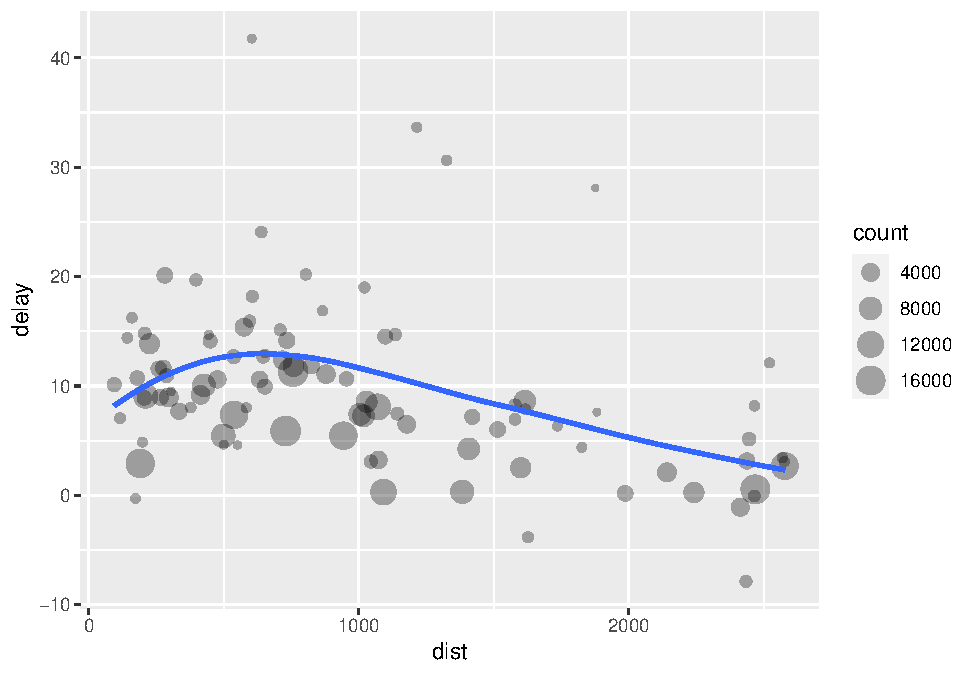
\includegraphics{mind2_files/figure-latex/unnamed-chunk-35-1.pdf}

Outra forma de atacar o problema seria:

\begin{Shaded}
\begin{Highlighting}[]
\NormalTok{delays }\OtherTok{\textless{}{-}}\NormalTok{ flights }\SpecialCharTok{\%\textgreater{}\%} 
  \FunctionTok{group\_by}\NormalTok{(dest) }\SpecialCharTok{\%\textgreater{}\%} 
  \FunctionTok{summarise}\NormalTok{(}
    \AttributeTok{count =} \FunctionTok{n}\NormalTok{(),}
    \AttributeTok{dist =} \FunctionTok{mean}\NormalTok{(distance, }\AttributeTok{na.rm =} \ConstantTok{TRUE}\NormalTok{),}
    \AttributeTok{delay =} \FunctionTok{mean}\NormalTok{(arr\_delay, }\AttributeTok{na.rm =} \ConstantTok{TRUE}\NormalTok{)}
\NormalTok{  ) }\SpecialCharTok{\%\textgreater{}\%} 
  \FunctionTok{filter}\NormalTok{(count }\SpecialCharTok{\textgreater{}} \DecValTok{20}\NormalTok{, dest }\SpecialCharTok{!=} \StringTok{"HNL"}\NormalTok{)}
\end{Highlighting}
\end{Shaded}

Quando utilizamos estes verbos e esta forma de trabalhar foca-se nas
transformações e não no que está sendo transformado o que torna o código
mais legível.

\textbf{Vejamos agora o argumento \emph{na.rm ( )}}

Este argumento remove os valores NA antes dos cálculos de agregados.

Assim, se quisermos retirar os voos cancelados teriamos:

\begin{Shaded}
\begin{Highlighting}[]
\NormalTok{not\_cancelled }\OtherTok{\textless{}{-}}\NormalTok{ flights }\SpecialCharTok{\%\textgreater{}\%} 
  \FunctionTok{filter}\NormalTok{(}\SpecialCharTok{!}\FunctionTok{is.na}\NormalTok{(dep\_delay), }\SpecialCharTok{!}\FunctionTok{is.na}\NormalTok{(arr\_delay))}

\NormalTok{not\_cancelled }\SpecialCharTok{\%\textgreater{}\%} 
  \FunctionTok{group\_by}\NormalTok{(year, month, day) }\SpecialCharTok{\%\textgreater{}\%} 
  \FunctionTok{summarise}\NormalTok{(}\AttributeTok{mean =} \FunctionTok{mean}\NormalTok{(dep\_delay))}
\end{Highlighting}
\end{Shaded}

\begin{verbatim}
## # A tibble: 365 x 4
## # Groups:   year, month [12]
##     year month   day  mean
##    <int> <int> <int> <dbl>
##  1  2013     1     1 11.4 
##  2  2013     1     2 13.7 
##  3  2013     1     3 10.9 
##  4  2013     1     4  8.97
##  5  2013     1     5  5.73
##  6  2013     1     6  7.15
##  7  2013     1     7  5.42
##  8  2013     1     8  2.56
##  9  2013     1     9  2.30
## 10  2013     1    10  2.84
## # ... with 355 more rows
\end{verbatim}

\hypertarget{contagens}{%
\subsection{Contagens}\label{contagens}}

Sempre que fazemos um resumo ou agregação é interessante adicionar uma
contagem \emph{n()} ou a contagem de não NAs, -sum(! is.na(x))\_.

Exemplo: Ver os voos pelo identificador do avião tailnum.

\begin{Shaded}
\begin{Highlighting}[]
\NormalTok{delays }\OtherTok{\textless{}{-}}\NormalTok{ not\_cancelled }\SpecialCharTok{\%\textgreater{}\%} 
  \FunctionTok{group\_by}\NormalTok{(tailnum) }\SpecialCharTok{\%\textgreater{}\%} 
  \FunctionTok{summarise}\NormalTok{(}
    \AttributeTok{delay =} \FunctionTok{mean}\NormalTok{(arr\_delay)}
\NormalTok{  )}

\FunctionTok{ggplot}\NormalTok{(}\AttributeTok{data =}\NormalTok{ delays, }\AttributeTok{mapping =} \FunctionTok{aes}\NormalTok{(}\AttributeTok{x =}\NormalTok{ delay)) }\SpecialCharTok{+} 
  \FunctionTok{geom\_freqpoly}\NormalTok{(}\AttributeTok{binwidth =} \DecValTok{10}\NormalTok{)}
\end{Highlighting}
\end{Shaded}

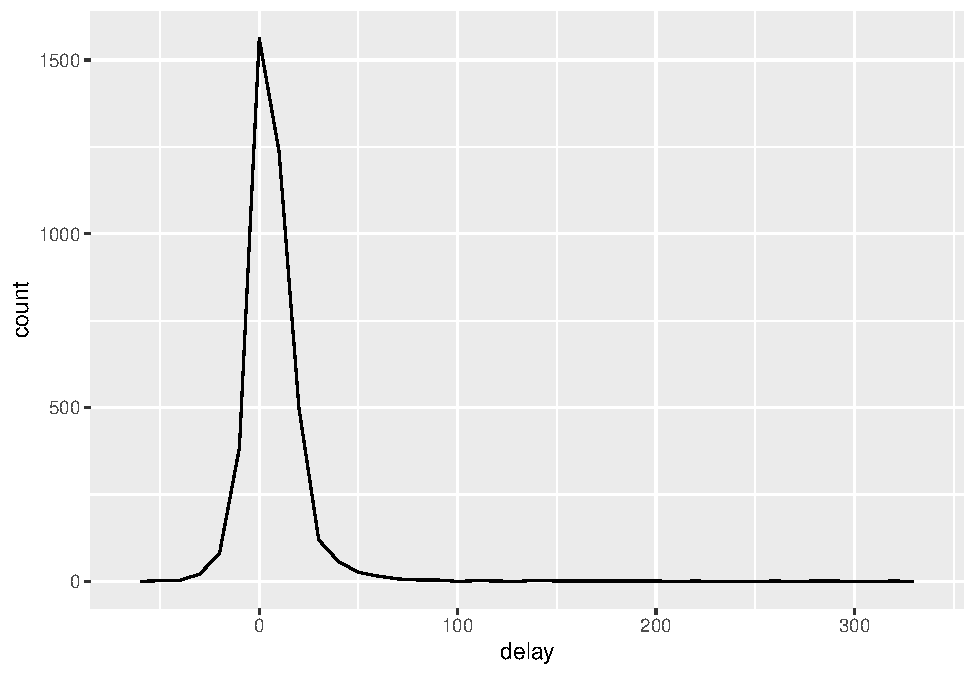
\includegraphics{mind2_files/figure-latex/unnamed-chunk-38-1.pdf}

A estória pode melhorar se você buscar ver gráficos de dispersão\ldots{}
faça depois.

\hypertarget{outras-funuxe7uxf5es-auxiliares-de-sumuxe1rio}{%
\subsection{Outras funções auxiliares de
sumário}\label{outras-funuxe7uxf5es-auxiliares-de-sumuxe1rio}}

Há varia medidas de posição como média, \emph{mean(x)} e mediana,
\emph{median(x)}.

Algumas vezes combinamos agregação com seleções lógicas

Exemplo:

\begin{Shaded}
\begin{Highlighting}[]
\NormalTok{not\_cancelled }\SpecialCharTok{\%\textgreater{}\%} 
  \FunctionTok{group\_by}\NormalTok{(year, month, day) }\SpecialCharTok{\%\textgreater{}\%} 
  \FunctionTok{summarise}\NormalTok{(}
    \AttributeTok{avg\_delay1 =} \FunctionTok{mean}\NormalTok{(arr\_delay),}
    \AttributeTok{avg\_delay2 =} \FunctionTok{mean}\NormalTok{(arr\_delay[arr\_delay }\SpecialCharTok{\textgreater{}} \DecValTok{0}\NormalTok{]) }\CommentTok{\# the average positive delay}
\NormalTok{  )}
\end{Highlighting}
\end{Shaded}

\begin{verbatim}
## # A tibble: 365 x 5
## # Groups:   year, month [12]
##     year month   day avg_delay1 avg_delay2
##    <int> <int> <int>      <dbl>      <dbl>
##  1  2013     1     1     12.7         32.5
##  2  2013     1     2     12.7         32.0
##  3  2013     1     3      5.73        27.7
##  4  2013     1     4     -1.93        28.3
##  5  2013     1     5     -1.53        22.6
##  6  2013     1     6      4.24        24.4
##  7  2013     1     7     -4.95        27.8
##  8  2013     1     8     -3.23        20.8
##  9  2013     1     9     -0.264       25.6
## 10  2013     1    10     -5.90        27.3
## # ... with 355 more rows
\end{verbatim}

\begin{itemize}
\tightlist
\item
  Medidas de dispersão
\end{itemize}

\emph{sd(x)}, \emph{IQR(x)},\emph{mad(x)} são medidas para verificar
outliers.

\begin{Shaded}
\begin{Highlighting}[]
\CommentTok{\# Porque as variações para algumas destinações são maiores que as outras?}
\NormalTok{not\_cancelled }\SpecialCharTok{\%\textgreater{}\%} 
  \FunctionTok{group\_by}\NormalTok{(dest) }\SpecialCharTok{\%\textgreater{}\%} 
  \FunctionTok{summarise}\NormalTok{(}\AttributeTok{distance\_sd =} \FunctionTok{sd}\NormalTok{(distance)) }\SpecialCharTok{\%\textgreater{}\%} 
  \FunctionTok{arrange}\NormalTok{(}\FunctionTok{desc}\NormalTok{(distance\_sd))}
\end{Highlighting}
\end{Shaded}

\begin{verbatim}
## # A tibble: 104 x 2
##    dest  distance_sd
##    <chr>       <dbl>
##  1 EGE         10.5 
##  2 SAN         10.4 
##  3 SFO         10.2 
##  4 HNL         10.0 
##  5 SEA          9.98
##  6 LAS          9.91
##  7 PDX          9.87
##  8 PHX          9.86
##  9 LAX          9.66
## 10 IND          9.46
## # ... with 94 more rows
\end{verbatim}

\begin{itemize}
\tightlist
\item
  Medidas de ordem
\end{itemize}

\emph{min(x)}, \emph{quantile(x)}, \emph{max(x)}

Quantile é uma generalização da mediana, exemplo \emph{quantile(x,
0.25)} encontrará o valor de x que é maior que 25\% dos valores e menor
que os 75\% restantes.

\begin{Shaded}
\begin{Highlighting}[]
\CommentTok{\# Quando o primeiro e último voo partem cada dia?}
\NormalTok{not\_cancelled }\SpecialCharTok{\%\textgreater{}\%} 
  \FunctionTok{group\_by}\NormalTok{(year, month, day) }\SpecialCharTok{\%\textgreater{}\%} 
  \FunctionTok{summarise}\NormalTok{(}
    \AttributeTok{first =} \FunctionTok{min}\NormalTok{(dep\_time),}
    \AttributeTok{last =} \FunctionTok{max}\NormalTok{(dep\_time)}
\NormalTok{  )}
\end{Highlighting}
\end{Shaded}

\begin{verbatim}
## # A tibble: 365 x 5
## # Groups:   year, month [12]
##     year month   day first  last
##    <int> <int> <int> <int> <int>
##  1  2013     1     1   517  2356
##  2  2013     1     2    42  2354
##  3  2013     1     3    32  2349
##  4  2013     1     4    25  2358
##  5  2013     1     5    14  2357
##  6  2013     1     6    16  2355
##  7  2013     1     7    49  2359
##  8  2013     1     8   454  2351
##  9  2013     1     9     2  2252
## 10  2013     1    10     3  2320
## # ... with 355 more rows
\end{verbatim}

\begin{itemize}
\tightlist
\item
  medidas de posicionamento
\end{itemize}

\emph{first(x)}, \emph{nth(x,2)}, \emph{last(x)}

Estes são outros modos de fazer \emph{x{[}1{]}}, \emph{x{[}2{]}} e
\emph{x{[}length(x){]}}

exemplo:

\begin{Shaded}
\begin{Highlighting}[]
\NormalTok{not\_cancelled }\SpecialCharTok{\%\textgreater{}\%} 
  \FunctionTok{group\_by}\NormalTok{(year, month, day) }\SpecialCharTok{\%\textgreater{}\%} 
  \FunctionTok{summarise}\NormalTok{(}
    \AttributeTok{first\_dep =} \FunctionTok{first}\NormalTok{(dep\_time), }
    \AttributeTok{last\_dep =} \FunctionTok{last}\NormalTok{(dep\_time)}
\NormalTok{  )}
\end{Highlighting}
\end{Shaded}

\begin{verbatim}
## # A tibble: 365 x 5
## # Groups:   year, month [12]
##     year month   day first_dep last_dep
##    <int> <int> <int>     <int>    <int>
##  1  2013     1     1       517     2356
##  2  2013     1     2        42     2354
##  3  2013     1     3        32     2349
##  4  2013     1     4        25     2358
##  5  2013     1     5        14     2357
##  6  2013     1     6        16     2355
##  7  2013     1     7        49     2359
##  8  2013     1     8       454     2351
##  9  2013     1     9         2     2252
## 10  2013     1    10         3     2320
## # ... with 355 more rows
\end{verbatim}

\hypertarget{mais-sobre-contagens}{%
\subsection{Mais sobre contagens}\label{mais-sobre-contagens}}

Vimos que \emph{n( )} não tem argumentos e retorna com o tamanho de um
grupo.

Para contar o número de valores presentes utilize: \emph{sum(!is.na(x))}

Para obter a contagem de valores únicos no grupo utilize:
\emph{n\_distinct(x)}

Exemplo: Quais os destinos que tem mais transportadores?

\begin{Shaded}
\begin{Highlighting}[]
\NormalTok{not\_cancelled }\SpecialCharTok{\%\textgreater{}\%} 
  \FunctionTok{group\_by}\NormalTok{(dest) }\SpecialCharTok{\%\textgreater{}\%} 
  \FunctionTok{summarise}\NormalTok{(}\AttributeTok{carriers =} \FunctionTok{n\_distinct}\NormalTok{(carrier)) }\SpecialCharTok{\%\textgreater{}\%} 
  \FunctionTok{arrange}\NormalTok{(}\FunctionTok{desc}\NormalTok{(carriers))}
\end{Highlighting}
\end{Shaded}

\begin{verbatim}
## # A tibble: 104 x 2
##    dest  carriers
##    <chr>    <int>
##  1 ATL          7
##  2 BOS          7
##  3 CLT          7
##  4 ORD          7
##  5 TPA          7
##  6 AUS          6
##  7 DCA          6
##  8 DTW          6
##  9 IAD          6
## 10 MSP          6
## # ... with 94 more rows
\end{verbatim}

Contagens são tão importantes que o \emph{dplyr} nos oferece
facilidades.

\begin{Shaded}
\begin{Highlighting}[]
\NormalTok{not\_cancelled }\SpecialCharTok{\%\textgreater{}\%} 
  \FunctionTok{count}\NormalTok{(dest)}
\end{Highlighting}
\end{Shaded}

\begin{verbatim}
## # A tibble: 104 x 2
##    dest      n
##    <chr> <int>
##  1 ABQ     254
##  2 ACK     264
##  3 ALB     418
##  4 ANC       8
##  5 ATL   16837
##  6 AUS    2411
##  7 AVL     261
##  8 BDL     412
##  9 BGR     358
## 10 BHM     269
## # ... with 94 more rows
\end{verbatim}

Podes opcionalmente prover uma variável de peso.

exemplo: Utilizando a função para omar as distâncias percorridas por
cada avião.

\begin{Shaded}
\begin{Highlighting}[]
\NormalTok{not\_cancelled }\SpecialCharTok{\%\textgreater{}\%} 
  \FunctionTok{count}\NormalTok{(tailnum, }\AttributeTok{wt =}\NormalTok{ distance)}
\end{Highlighting}
\end{Shaded}

\begin{verbatim}
## # A tibble: 4,037 x 2
##    tailnum      n
##    <chr>    <dbl>
##  1 D942DN    3418
##  2 N0EGMQ  239143
##  3 N10156  109664
##  4 N102UW   25722
##  5 N103US   24619
##  6 N104UW   24616
##  7 N10575  139903
##  8 N105UW   23618
##  9 N107US   21677
## 10 N108UW   32070
## # ... with 4,027 more rows
\end{verbatim}

Pode-se combinar contagens com testes: sum(x\textgreater10), mean(y==0).

exemplo: quantos voos partiram antes das 5:00 h A.M.?

\begin{Shaded}
\begin{Highlighting}[]
\NormalTok{not\_cancelled }\SpecialCharTok{\%\textgreater{}\%} 
  \FunctionTok{group\_by}\NormalTok{(year, month, day) }\SpecialCharTok{\%\textgreater{}\%} 
  \FunctionTok{summarise}\NormalTok{(}\AttributeTok{n\_early =} \FunctionTok{sum}\NormalTok{(dep\_time }\SpecialCharTok{\textless{}} \DecValTok{500}\NormalTok{))}
\end{Highlighting}
\end{Shaded}

\begin{verbatim}
## # A tibble: 365 x 4
## # Groups:   year, month [12]
##     year month   day n_early
##    <int> <int> <int>   <int>
##  1  2013     1     1       0
##  2  2013     1     2       3
##  3  2013     1     3       4
##  4  2013     1     4       3
##  5  2013     1     5       3
##  6  2013     1     6       2
##  7  2013     1     7       2
##  8  2013     1     8       1
##  9  2013     1     9       3
## 10  2013     1    10       3
## # ... with 355 more rows
\end{verbatim}

ou que proporção dos voos atrasou mais de uma hora?

\begin{Shaded}
\begin{Highlighting}[]
\NormalTok{not\_cancelled }\SpecialCharTok{\%\textgreater{}\%} 
  \FunctionTok{group\_by}\NormalTok{(year, month, day) }\SpecialCharTok{\%\textgreater{}\%} 
  \FunctionTok{summarise}\NormalTok{(}\AttributeTok{hour\_perc =} \FunctionTok{mean}\NormalTok{(arr\_delay }\SpecialCharTok{\textgreater{}} \DecValTok{60}\NormalTok{))}
\end{Highlighting}
\end{Shaded}

\begin{verbatim}
## # A tibble: 365 x 4
## # Groups:   year, month [12]
##     year month   day hour_perc
##    <int> <int> <int>     <dbl>
##  1  2013     1     1    0.0722
##  2  2013     1     2    0.0851
##  3  2013     1     3    0.0567
##  4  2013     1     4    0.0396
##  5  2013     1     5    0.0349
##  6  2013     1     6    0.0470
##  7  2013     1     7    0.0333
##  8  2013     1     8    0.0213
##  9  2013     1     9    0.0202
## 10  2013     1    10    0.0183
## # ... with 355 more rows
\end{verbatim}

\end{document}
